% !TeX spellcheck = en_GB
% !TeX program = pdflatex
%
% LuxSleek-CV 1.1 LaTeX template
% Author: Andreï V. Kostyrka, University of Luxembourg
%
% 1.1: added tracking and letter-spacing for prettier lower caps, added `~` for language levels
% 1.0: initial release
%
% This template fills the gap in the available variety of templates
% by proposing something that is not a custom class, not using any
% hard-coded settings deeply hidden in style files, and provides
% a handful of custom command definitions that are as transparent as it gets.
% Developed at the University of Luxembourg.
%
% *NOTHING IS HARCODED, and never should be.*
%
% Target audience: applicants in the IT industry, or business in general
%
% The main strength of this template is, it explicitly showcases how
% to break the flow of text to achieve the most flexible right alignment
% of dates for multiple configurations.

\documentclass[11pt, a4paper]{article} 
\usepackage{fontawesome}
\usepackage[T1]{fontenc}     % We are using pdfLaTeX,
\usepackage[utf8]{inputenc}  % hence this preparation
\usepackage[british]{babel}  
\usepackage[left = 0mm, right = 0mm, top = 0mm, bottom = 0mm]{geometry}
\usepackage[stretch = 25, shrink = 25, tracking=true, letterspace=30]{microtype}  
\usepackage{graphicx}        % To insert pictures
\usepackage{xcolor}          % To add colour to the document

\usepackage{enumitem}        % To redefine spacing in lists
\setlist{parsep = 0pt, topsep = 0pt, partopsep = 1pt, itemsep = 1pt, leftmargin = 6mm}

\usepackage[sfdefault]{FiraSans}        % Change this to use any font, but keep it simple
\renewcommand{\familydefault}{\sfdefault}
%\usepackage{fetamont}

\definecolor{cvblue}{HTML}{304263}

%%%%%%% USER COMMAND DEFINITIONS %%%%%%%%%%%%%%%%%%%%%%%%%%%
% These are the real workhorses of this template
\newcommand{\dates}[1]{\hfill\mbox{\textbf{#1}}} % Bold stuff that doesn’t got broken into lines
\newcommand{\is}{\par\vskip.5ex plus .4ex} % Item spacing
\newcommand{\smaller}[1]{{\small$\diamond$\ #1}}
\newcommand{\headleft}[1]{\vspace*{3ex}\textsc{\textbf{#1}}\par%
    \vspace*{-1.5ex}\hrulefill\par\vspace*{0.7ex}}
\newcommand{\headright}[1]{\vspace*{2.5ex}\textsc{\Large\color{cvblue}#1}\par%
     \vspace*{-2ex}{\color{cvblue}\hrulefill}\par}
%%%%%%%%%%%%%%%%%%%%%%%%%%%%%%%%%%%%%%%%%%%%%%%%%%%%%%%%%%%%

\usepackage[colorlinks = true, urlcolor = white, linkcolor = white]{hyperref}

\begin{document}

% Style definitions -- killing the unnecessary space and adding the skips explicitly
\setlength{\topskip}{0pt}
\setlength{\parindent}{0pt}
\setlength{\parskip}{0pt}
\setlength{\fboxsep}{0pt}
\pagestyle{empty}
\raggedbottom

\begin{minipage}[t]{0.33\textwidth} %% Left column -- outer definition
%  Left column -- top dark rectangle
\colorbox{cvblue}{\begin{minipage}[t][5mm][t]{\textwidth}\null\hfill\null\end{minipage}}

\vspace{-.2ex} % Eliminates the small gap
\colorbox{cvblue!90}{\color{white}  %% LEFT BOX
\kern0.09\textwidth\relax% Left margin provided explicitly
\begin{minipage}[t][293mm][t]{0.82\textwidth}
\raggedright
\vspace*{2.5ex}

\Large Jason \textbf{\textsc{Felice}} \normalsize

% Centering without extra vertical spacing
\null\hfill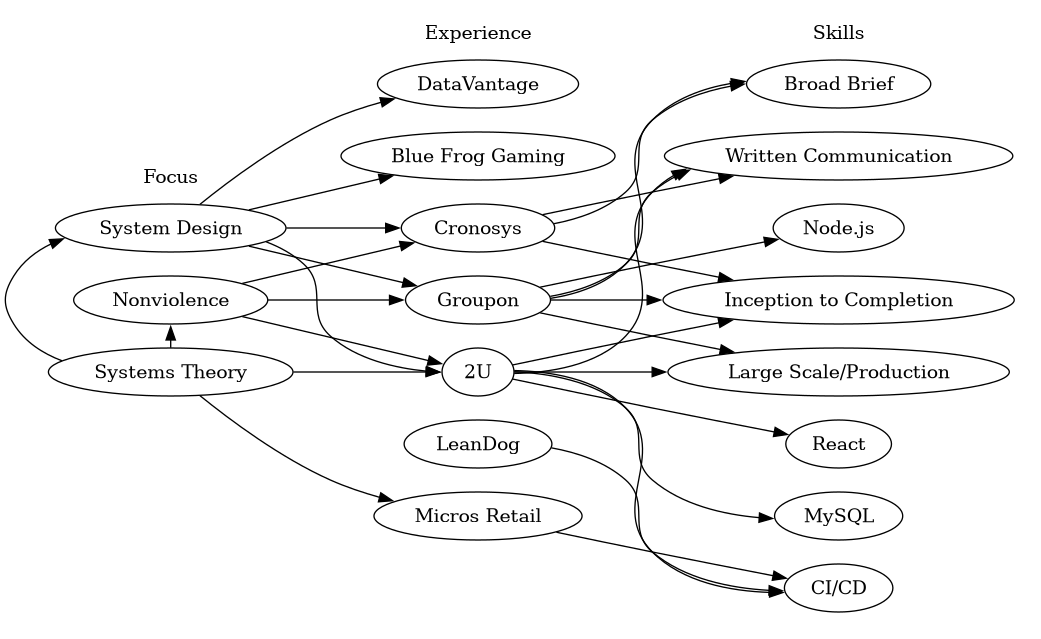
\includegraphics[width=0.65\textwidth]{stack_graph.png}\hfill\null

\vspace*{0.5ex} % Extra space after the picture

\headleft{Goal}

Bring all voices into a sustainable software development practice;
collaborate, facilitate, and mentor; celebrate beautiful code, geek joy,
emergent behavior, and math.

\headleft{Profile}

I've been: a consultant, a tech lead, an architecture reviewer, a one-person
software department, a business analyst, a process hacker, a network administrator,
a game developer, a salesperson, the Person Who Automated Themself Out of a Job, a web
developer, an inventor of algorithmic solutions, an evangelist, the Chief Technology Officer,
the Person Who Made It Faster With Assembly, an Open Source contributor, and barista.

\headleft{Contact details}
\small % To fit more content
\faAt\ {\small jason.m.felice@gmail.com} \\[0.4ex]
\faPhone\ +1\,216\,466\,4122 \\[0.5ex]
\faGithub\ \href{https://github.com/eraserhd}{github.com/eraserhd} \\[0.1ex]
\faEnvelope\ 25100 Farringdon Ave \\[0.5ex]
Euclid, Ohio 44132, USA
\normalsize

\headleft{Skills}

\begin{itemize}
\item Clojure, Java
\item Go
\item C, C++, Objective-C
\item iOS, Android
\item Erlang, Elixir
\item Javascript, Python
\end{itemize} 

\end{minipage}%
\kern0.09\textwidth\relax%%Right margin provided explicitly to stretch the colourbox
}
\end{minipage}% Right column
\hskip2.5em% Left margin for the white area
\begin{minipage}[t]{0.56\textwidth}

\setlength{\parskip}{0.8ex}% Adds spaces between paragraphs; use \\ to add new lines without this space. Shrink this amount to fit more data vertically

\vspace{2ex}

\headright{Large System Builder}
\null\hfill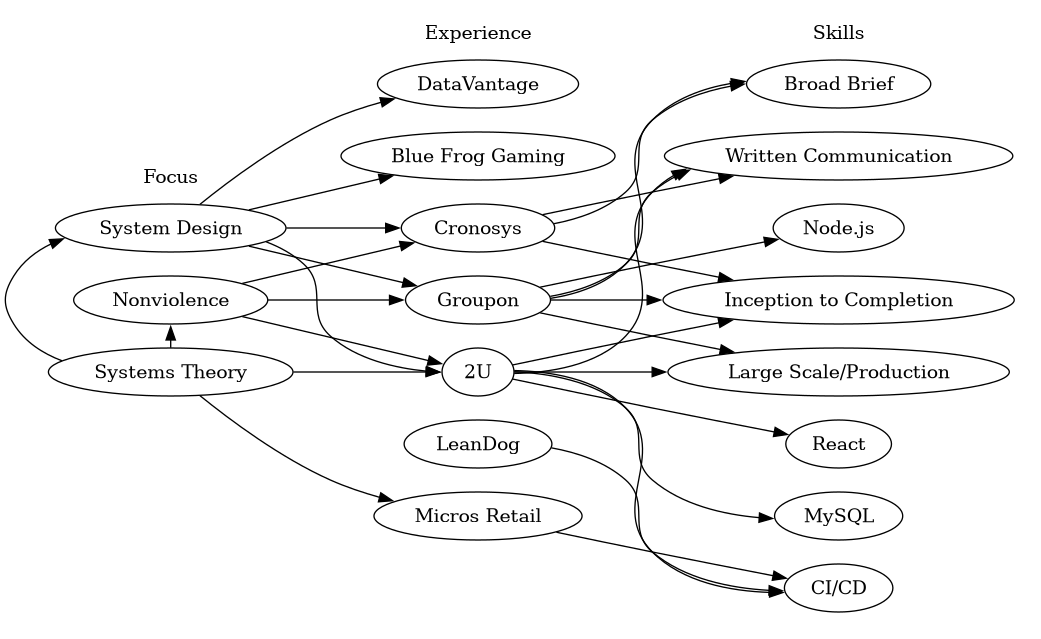
\includegraphics[width=\textwidth]{stack_graph.png}\hfill\null

\headright{Experience}

\textsc{Software Engineer IV} at \textit{2U}  \dates{2016.06--2025.04} \\
\smaller{Automated new program standup} \\
\smaller{Brought an acquired company's tech stack up to 2U standards} \\
\smaller{Maintained core systems and proposed technical direction}

\is % Item spacing -- defined in the preamble
\textsc{Software Engineer IV} at \textit{Groupon}  \dates{2013.02--2016.06} \\
\smaller{Implemented and delivered new homepage} \\
\smaller{Designed and delivered Points retention program} \\
\smaller{Broke a delivery-limiting stalemate between tech and purchasing}

\is
\textsc{iOS+Android Developer} at \textit{LeanDog} \dates{2011.11--2013.02} \\
\smaller{Maintained iOS application and ported it to Android}

\is
\textsc{Software Engineer} at \textit{Blue Frog Gaming} \dates{2010.09--2011.11} \\ 
\smaller{Designed and delivered Polar Puzzles and Ghost Chicken iPad games} \\
\smaller{Maintained Hearts and Spades iPad games and network servers}

\is
\textsc{Senior Software Engineer} at \textit{Micros Retail} \dates{2007.04--2010.09} \\
\smaller{Maintained DAS and XPay credit authorization systems} \\
\smaller{Implemented processes dramatically reducing delivery failures}

\is
\textsc{Chief Technology Officer} at \textit{Cronosys, LLC} \dates{2000.01--2007.04} \\
\smaller{Made a bet on web technology for internal business apps} \\
\smaller{Consulted, quoted, and delivered many projects on many tech stacks}

\is
\textsc{Consultant} at \textit{The Baldwin Group} \dates{1997.03--2000.01}\\  
\smaller{Consulted on PC-related issues} \\
\smaller{Maintained Mayor's Court software}

\is
\textsc{Programmer/Analyst} at \textit{DataVantage} \dates{1994.02--1997.03} \\
\smaller{Automated third shift data communications} \\
\smaller{Implemented new credit authorization system} \\
\smaller{Maintained point-of-sale software}
\end{minipage}

\end{document}
